\documentclass[
% -- opções da classe memoir --
article,			% indica que é um artigo acadêmico
11pt,				% tamanho da fonte
oneside,			% para impressão apenas no verso. Oposto a twoside
a4paper,			% tamanho do papel. 
% -- opções da classe abntex2 --
%chapter=TITLE,		% títulos de capítulos convertidos em letras maiúsculas
%section=TITLE,		% títulos de seções convertidos em letras maiúsculas
%subsection=TITLE,	% títulos de subseções convertidos em letras maiúsculas
%subsubsection=TITLE % títulos de subsubseções convertidos em letras maiúsculas
% -- opções do pacote babel --
english,			% idioma adicional para hifenização
brazil,				% o último idioma é o principal do documento
sumario=tradicional
]{abntex2}

%teste do joao
\usepackage{C:/Users/Lucca/GoogleDrive/Latex/mystyle}
%% Espaçamento simples
\SingleSpacing

\title{Artigo Macroeconometria}
\autor{Lucca Simeoni Pavan
	\thanks{Doutorando em Desenvolvimento Econômico, PPDGE/UFPR - warrenjax@gmail.com}\and João Carlos de Carvalho\thanks{Doutorando em Desenvolvimento Econômico, PPDGE/UFPR - joaocarlos\_carva@hotmail.com}\and Marcos Minoru Hasegawa\thanks{Professor do Departamento de Economia da UFPR e do PPGDE/UFPR}}
\local{Brasil}
\data{\today}
% ---

% ----
% Início do documento
% ----
\begin{document}
	
\maketitle
\mainmatter
%\input{resumo}
\section{Introdução}
knnnk
\documentclass[]{article}
\usepackage{lmodern}
\usepackage{amssymb,amsmath}
\usepackage{ifxetex,ifluatex}
\usepackage{fixltx2e} % provides \textsubscript
\ifnum 0\ifxetex 1\fi\ifluatex 1\fi=0 % if pdftex
  \usepackage[T1]{fontenc}
  \usepackage[utf8]{inputenc}
\else % if luatex or xelatex
  \ifxetex
    \usepackage{mathspec}
  \else
    \usepackage{fontspec}
  \fi
  \defaultfontfeatures{Ligatures=TeX,Scale=MatchLowercase}
\fi
% use upquote if available, for straight quotes in verbatim environments
\IfFileExists{upquote.sty}{\usepackage{upquote}}{}
% use microtype if available
\IfFileExists{microtype.sty}{%
\usepackage{microtype}
\UseMicrotypeSet[protrusion]{basicmath} % disable protrusion for tt fonts
}{}
\usepackage[margin=1in]{geometry}
\usepackage{hyperref}
\hypersetup{unicode=true,
            pdfborder={0 0 0},
            breaklinks=true}
\urlstyle{same}  % don't use monospace font for urls
\usepackage{longtable,booktabs}
\usepackage{graphicx,grffile}
\makeatletter
\def\maxwidth{\ifdim\Gin@nat@width>\linewidth\linewidth\else\Gin@nat@width\fi}
\def\maxheight{\ifdim\Gin@nat@height>\textheight\textheight\else\Gin@nat@height\fi}
\makeatother
% Scale images if necessary, so that they will not overflow the page
% margins by default, and it is still possible to overwrite the defaults
% using explicit options in \includegraphics[width, height, ...]{}
\setkeys{Gin}{width=\maxwidth,height=\maxheight,keepaspectratio}
\IfFileExists{parskip.sty}{%
\usepackage{parskip}
}{% else
\setlength{\parindent}{0pt}
\setlength{\parskip}{6pt plus 2pt minus 1pt}
}
\setlength{\emergencystretch}{3em}  % prevent overfull lines
\providecommand{\tightlist}{%
  \setlength{\itemsep}{0pt}\setlength{\parskip}{0pt}}
\setcounter{secnumdepth}{5}
% Redefines (sub)paragraphs to behave more like sections
\ifx\paragraph\undefined\else
\let\oldparagraph\paragraph
\renewcommand{\paragraph}[1]{\oldparagraph{#1}\mbox{}}
\fi
\ifx\subparagraph\undefined\else
\let\oldsubparagraph\subparagraph
\renewcommand{\subparagraph}[1]{\oldsubparagraph{#1}\mbox{}}
\fi

%%% Use protect on footnotes to avoid problems with footnotes in titles
\let\rmarkdownfootnote\footnote%
\def\footnote{\protect\rmarkdownfootnote}

%%% Change title format to be more compact
\usepackage{titling}

% Create subtitle command for use in maketitle
\newcommand{\subtitle}[1]{
  \posttitle{
    \begin{center}\large#1\end{center}
    }
}

\setlength{\droptitle}{-2em}
  \title{}
  \pretitle{\vspace{\droptitle}}
  \posttitle{}
  \author{}
  \preauthor{}\postauthor{}
  \date{}
  \predate{}\postdate{}

\setlength\parindent{24pt}
\usepackage[english, brazil]{babel}
\usepackage[utf8]{inputenc}
\usepackage{longtable}
\usepackage{booktabs}
\usepackage{indentfirst}

\begin{document}

\section{Revisão de Literatura: Estudos de volatilidade no mercado
financeiro
brasileiro}\label{revisao-de-literatura-estudos-de-volatilidade-no-mercado-financeiro-brasileiro}

Moreira e Lemgruber (2004) investigaram o uso de dados de alta
frequência na estimação da volatilidade diária e intradiária do IBOVESPA
e no cálculo do valor em risco (VaR). Para isso usaram os modelos GARCH
e EGARCH em conjunto com métodos determinísticos de filtragem de
sazonalidade para a previsão da volatilidade e do VaR intradiários. Os
autores compararam seus resultados com o método não paramétrico e no
cálculo do VaR diário, dois métodos foram usados. O primeiro utiliza o
desvio padrão amostral com janela móvel e o segundo usa alisamento
exponencial. No cálculo do VaR diário, os dois métodos usados baseados
em informações intradiárias apresentaram bom desempenho. Ao calcularem o
VaR intradiário, seus resultados mostraram que a filtragem do padrão
sazonal é indispensável à obtenção de resultados satisfatórios por meio
dos modelos GARCH e EGARCH. A série utilizada pelos autores é o índice
IBOVESPA, registrados a cada 15 minutos durante o período de 06/04/1998
a 19/07/2001 e utilizaram o retorno logarítmico para as estimações. Os
autores também concluíram que o filtro de sazonalidade do intervalo
intradiário é mais importante para melhorar os resultados das estimações
do que o filtro referente ao dia da semana.

Carvalho et al. (2006) estimaram a volatilidade diária dos cinco ativos
amis negociados na bolsa de valores de São Paulo (na época BOVESPA e
BM\&F eram separadas). Os autores utilizaram dados intradiários e
utilizaram o estmador de variância realizada. Os autores concluíram que
os retornos diários padronizados pela volatilidade realizada são
aproximadamente normais. Também concluíram que as log-volatilidades
também apresentam distribuições bem próximas da normal. Em contraposição
com a literatura corrente até então, não encontraram evidências de
memória de longo prazo na série de volatilidade e um modelo de memória
curta foi suficiente para os autores modelarem e preverem as séries
diárias de volatilidade. Os modelo usados pelos autores foram o retorno
logarítimico padrozinado, EWMA, GARCH, EGARCH e GJR-GARCH.

Ceretta et al. (2011) inestigaram como a especificação da distribuição
influencia a performandce da previsão da volatilidade em dados
intradiários do IBovespa, usando o modelo APARCH. As previsões dos
autores foram realizadas supondo seis distribuições dinstintas: normal,
normal assimétrica, \emph{t-student}, \emph{t-student} assimétrica,
generalizada e generalizada assimétrica. Os resultados obtidos mostraram
que o modelo com distribuição \emph{t-student} assimétrica foi o que
melhor se ajustou aos dados dentro da amostra, porém, na previsão fora
da amostra, o modelo com distribuição normal apresentou melhor
desempenho.

Ceretta et al. (2011) encontraram também que uma modelagem feita a
partir de um asérie longa pode incorporar efeitos atípicos no modelo,
viesando a previsão. Os autores apoantam como uma possível solução
realizar um ajuste do modelo utilizando uma série menor, com menos
efeitos esporádicos, em que, segundo eles, a previsão poderia ter um
comportamento amis aproximado ao habitual para a série, o que
minimizaria o efeito de eventuais variações acentudas. Outro fato
destacado pelos autores é que o modelo que melhor se ajusta, nem sempre
fornecerá amelhor previsão. Isto, conforme Ceretta et al. (2011) ,
ressalta a importância da comparação entre os modelos estudados fora da
amostra para encontrar o modelo que melhor prevê o comportamento futuro
da série. a partir disso os autores sugerirm que o contexto
macroeconômico poderia influenciar tanto o ajuste quanto a previsão de
uma série financeira.

Junior e Pereira (2013) usaram dados intradiários com intervalo de tempo
de 5, 15 e 30 minutos para as ações mais comercializadas do índice
BOVESPA. Seu artigo analisou dois modelos para estimação e previsão da
volatilidade realizada: o modelo autorregressivo heterogÊneo de
volatilidade realizada (HAR-RV) e o modelo de amostragem de dados mistos
(MIDAS-RV). Os autores compararam previsões dentro e fora da amostra e
encontraram melhores resultados com o modelo MIDAS-RV para previsões
dentro da amostra. Para previsões fora da amostra não encontraram
diferença estatísticamente significativa entre os modelos. Por fim os
autores acharam evidência de que o uso de volatilidade realizada induz a
distribuições dos retornos padronizados próximas da normal.

Santos e Ziegelmann (2014) compararam diversos tipos de medidas de
volatilidade e seus modelos de previsão, das famílias de modelos
MIDAS-RV e HAR-RV. Realizaram comarações em temos da acurácia de
previsão da volatilidade fora da amostra e usaram também uma combinação
dos dois modelos. Para isso captaram dados intradiários do índice
IBOVESPA e calcularam medidas de volatilidade como variância realizada,
variação potência realizada e variação bi-potência realziada para serem
usados como regressores em ambos os modelos. Para a estimação usaram um
procedimento não paramétrico para mensurar separadamente a variação da
trajetória contínua da amostra e a parte de salto descontínuodo processo
de variação quadrático.Seus resultados em termos de erro quadrático
médio sigerem que regressores envolvendo medidas de volatilidade que são
robustos a saltos são melhores para previsão de volatilidade futura.
Encontraram ainda que previsõe sbaseadas nestes regressre não são
estatísticamente diferentes daqueles baseados em variância realizada.
Por fim, acharam que a performance de previsão das três abordagens são
estatísticamente equivalentes.

Vicente et al. (2014) examinaram se investidores possuem percepções
diferentes sobre a volatilidade diária de um ativo. Para isso, definiram
a volatilidade percebida pelo investidor como a distribuição dos
desvios-padrão dos retornos diários calculados de preços intradiários
coletados aleatoriamente. Os autores encontraram que esta distribuição
tem uma alto grau de dispersão, o que significa que diferentes
investidores podem não compartilhar a emsma opinião a respeito da
variabilidade do mesmo ativo. Entretanto, segundo Vicente et al. (2014)
a volatilidade de preços de fechamento é geralente menor que a mediana
da volatilidade percebida pelo investidor, enquanto a volatilidade de
preço de abertura é maior. Seus resultados indicaram que as
volatilidades usando amostras diárias tradicionais de retornos diários
podem não ser bons insumos de modelos financeiros, já que, conforme os
autores, eles podem não capturar adequadamente o risco em que os
investidores são expostos.

Ziegelmann, Borges e Caldeira (2014) exploraram diferentes estimadores
de matrix de covariância, tanto a condicional quanto a incondicional,
obtidas por dados intradiários. Tais medidas foram usadas para obter um
portfólio de variância mínima. Os dados foram coletados de forma
sincronizada e não sincronizada. Para fins de comparação os autores
também usaram dados diários. Em seu trabalho tambpem avaliaram as
performances fora da amostra dos índices obtidos de um portfólio de 30
ações comercializadas na BMF\&BOVESPA. Seus resultados mostraram que o
estimador da matrix de variância condicional dos retornos usando o
modelo escalar vt-VECH baseado em dados de alta frequÊncia leva a
melhoras substanciais de estimação, reduzindo o risco de portfólio,
aumentando o retorno médio ajustado pelo risco e reduzindo o
\emph{turnover} financeiro.

\begin{longtable}[]{@{}llll@{}}
\caption{Resumo dos estudos de volatilidade no mercado financeiro
brasileiro.}\tabularnewline
\toprule
\begin{minipage}[b]{0.17\columnwidth}\raggedright\strut
Autores\strut
\end{minipage} & \begin{minipage}[b]{0.17\columnwidth}\raggedright\strut
Objeto\strut
\end{minipage} & \begin{minipage}[b]{0.15\columnwidth}\raggedright\strut
Periodicidade\strut
\end{minipage} & \begin{minipage}[b]{0.23\columnwidth}\raggedright\strut
Método\strut
\end{minipage}\tabularnewline
\midrule
\endfirsthead
\toprule
\begin{minipage}[b]{0.17\columnwidth}\raggedright\strut
Autores\strut
\end{minipage} & \begin{minipage}[b]{0.17\columnwidth}\raggedright\strut
Objeto\strut
\end{minipage} & \begin{minipage}[b]{0.15\columnwidth}\raggedright\strut
Periodicidade\strut
\end{minipage} & \begin{minipage}[b]{0.23\columnwidth}\raggedright\strut
Método\strut
\end{minipage}\tabularnewline
\midrule
\endhead
\begin{minipage}[t]{0.17\columnwidth}\raggedright\strut
Moreira e Lemgruber (2004)\strut
\end{minipage} & \begin{minipage}[t]{0.17\columnwidth}\raggedright\strut
IBOVESPA\strut
\end{minipage} & \begin{minipage}[t]{0.15\columnwidth}\raggedright\strut
15 min e 1 dia\strut
\end{minipage} & \begin{minipage}[t]{0.23\columnwidth}\raggedright\strut
GARCH, EGARCH\strut
\end{minipage}\tabularnewline
\begin{minipage}[t]{0.17\columnwidth}\raggedright\strut
Carvalho et al. (2006)\strut
\end{minipage} & \begin{minipage}[t]{0.17\columnwidth}\raggedright\strut
Top 5 empresas IBOVESPA\strut
\end{minipage} & \begin{minipage}[t]{0.15\columnwidth}\raggedright\strut
15 min\strut
\end{minipage} & \begin{minipage}[t]{0.23\columnwidth}\raggedright\strut
EWMA, GARCH, EGARCH, GJR-GARCH, log retorno padronizado\strut
\end{minipage}\tabularnewline
\begin{minipage}[t]{0.17\columnwidth}\raggedright\strut
Ceretta et al. (2011)\strut
\end{minipage} & \begin{minipage}[t]{0.17\columnwidth}\raggedright\strut
IBOVESPA\strut
\end{minipage} & \begin{minipage}[t]{0.15\columnwidth}\raggedright\strut
15 min\strut
\end{minipage} & \begin{minipage}[t]{0.23\columnwidth}\raggedright\strut
APARCH\strut
\end{minipage}\tabularnewline
\begin{minipage}[t]{0.17\columnwidth}\raggedright\strut
Junior e Pereira (2013)\strut
\end{minipage} & \begin{minipage}[t]{0.17\columnwidth}\raggedright\strut
Top 5 empresas IBOVESPA\strut
\end{minipage} & \begin{minipage}[t]{0.15\columnwidth}\raggedright\strut
5, 15 e 30 min\strut
\end{minipage} & \begin{minipage}[t]{0.23\columnwidth}\raggedright\strut
HAR-RV e MIDAS-RV\strut
\end{minipage}\tabularnewline
\begin{minipage}[t]{0.17\columnwidth}\raggedright\strut
Morais et al. (2014)\strut
\end{minipage} & \begin{minipage}[t]{0.17\columnwidth}\raggedright\strut
Top 2 BMF\&BOVESPA\strut
\end{minipage} & \begin{minipage}[t]{0.15\columnwidth}\raggedright\strut
5 min\strut
\end{minipage} & \begin{minipage}[t]{0.23\columnwidth}\raggedright\strut
GARCH, EGARCH, CGARCH e TGARCH\strut
\end{minipage}\tabularnewline
\begin{minipage}[t]{0.17\columnwidth}\raggedright\strut
Santos e Ziegelmann (2014)\strut
\end{minipage} & \begin{minipage}[t]{0.17\columnwidth}\raggedright\strut
IBOVESPA\strut
\end{minipage} & \begin{minipage}[t]{0.15\columnwidth}\raggedright\strut
15 min\strut
\end{minipage} & \begin{minipage}[t]{0.23\columnwidth}\raggedright\strut
HAR, MIDAS e combinação HAR-MIDAS\strut
\end{minipage}\tabularnewline
\begin{minipage}[t]{0.17\columnwidth}\raggedright\strut
Vicente et al. (2014)\strut
\end{minipage} & \begin{minipage}[t]{0.17\columnwidth}\raggedright\strut
84 empresas da BMF\&BOVESPA\strut
\end{minipage} & \begin{minipage}[t]{0.15\columnwidth}\raggedright\strut
Amostragem aleatória de preços em um intervalo\strut
\end{minipage} & \begin{minipage}[t]{0.23\columnwidth}\raggedright\strut
Análise exploratória da Volatilidade Realizada\strut
\end{minipage}\tabularnewline
\begin{minipage}[t]{0.17\columnwidth}\raggedright\strut
Ziegelmann, Borges e Caldeira (2014)\strut
\end{minipage} & \begin{minipage}[t]{0.17\columnwidth}\raggedright\strut
Índice de 30 ações BMF\&BOVESPA\strut
\end{minipage} & \begin{minipage}[t]{0.15\columnwidth}\raggedright\strut
5 a 120 min\strut
\end{minipage} & \begin{minipage}[t]{0.23\columnwidth}\raggedright\strut
Covariância realizada, vt\_VECH escalar e MRK\strut
\end{minipage}\tabularnewline
\bottomrule
\end{longtable}

Fonte: Elaboração dos autores

\pagebreak

\section*{Referências}\label{referencias}
\addcontentsline{toc}{section}{Referências}

\setlength{\parindent}{0in}

\hypertarget{refs}{}
\hypertarget{ref-carvalho_modeling_2006}{}
CARVALHO, M. C.; FREIRE, M. A. S.; MEDEIROS, M. C.; SOUZA, L. R.
Modeling and Forecasting the Volatility of Brazilian Asset Returns: a
Realized Variance Approach. \textbf{Brazilian Review of Finance}, v. 4,
n. 1, p. 55--77, 2006. Disponível em:
\textless{}\url{http://bibliotecadigital.fgv.br/ojs/index.php/rbfin/article/view/1155}\textgreater{}.
Acesso em: 12/12/2016.

\hypertarget{ref-ceretta_intraday_2011}{}
CERETTA, P. S.; BARBA, F. G. DE; VIEIRA, K. M.; CASARIN, F. Intraday
volatility forecasting: analysis of alternative distributions.
\textbf{Brazilian Review of Finance}, v. 9, n. 2, p. 209--226, 2011.
Disponível em:
\textless{}\url{http://bibliotecadigital.fgv.br/ojs/index.php/rbfin/article/view/2586}\textgreater{}.
Acesso em: 12/12/2016.

\hypertarget{ref-junior_modeling_2013}{}
JUNIOR, M. V. W.; PEREIRA, P. L. V. Modeling and Forecasting of Realized
Volatility: Evidence from Brazil. \textbf{Brazilian Review of
Econometrics}, v. 31, n. 2, p. 315--337, 2013. Disponível em:
\textless{}\url{http://bibliotecadigital.fgv.br/ojs/index.php/bre/article/view/4056}\textgreater{}.
Acesso em: 12/12/2016.

\hypertarget{ref-morais_estimating_2014}{}
MORAIS, O.; VAL, F. DE F.; PINTO, A. C. F.; KL, M. C.; MACELLY.
Estimating the Volatility of Brazilian Equities using Garch-Type Models
and High-Frequency Volatility Measures. \textbf{Global Journal of
Management And Business Research}, v. 14, n. 5, 2014. Disponível em:
\textless{}\url{http://journalofbusiness.org/index.php/GJMBR/article/view/1520}\textgreater{}.
Acesso em: 12/12/2016.

\hypertarget{ref-moreira_o_2004}{}
MOREIRA, J. M. DE S.; LEMGRUBER, E. F. O uso de dados de alta freqüência
na estimação da volatilidade e do valor em risco para o IBOVESPA.
\textbf{Revista Brasileira de Economia}, v. 58, n. 1, p. 100--120, 2004.
Disponível em:
\textless{}\url{http://www.scielo.br/scielo.php?script=sci_abstract\&pid=S0034-71402004000100005\&lng=en\&nrm=iso\&tlng=pt}\textgreater{}.
Acesso em: 12/12/2016.

\hypertarget{ref-santos_volatility_2014}{}
SANTOS, D. G.; ZIEGELMANN, F. A. Volatility Forecasting via MIDAS, HAR
and their Combination: An Empirical Comparative Study for IBOVESPA.
\textbf{Journal of Forecasting}, v. 33, n. 4, p. 284--299, 2014.
Disponível em:
\textless{}\url{http://onlinelibrary.wiley.com/doi/10.1002/for.2287/abstract}\textgreater{}.
Acesso em: 12/12/2016.

\hypertarget{ref-vicente_assessing_2014}{}
VICENTE, J. V. M.; ARAUJO, G. S.; CASTRO, P. B. F. DE; TAVARES, F. N.
Assessing Day-to-Day Volatility: Does the Trading Time Matter?
\textbf{Brazilian Review of Finance}, v. 12, n. 1, p. 41--66, 2014.
Disponível em:
\textless{}\url{http://bibliotecadigital.fgv.br/ojs/index.php/rbfin/article/view/13483}\textgreater{}.
Acesso em: 12/12/2016.

\hypertarget{ref-ziegelmann_selection_2014}{}
ZIEGELMANN, F. A.; BORGES, B.; CALDEIRA, J. F. Selection of Minimum
Variance Portfolio Using Intraday Data: An Empirical Comparison Among
Different Realized Measures for BM\&FBovespa Data. \textbf{Brazilian
Review of Econometrics}, v. 35, n. 1, p. 23--46, 2014. Disponível em:
\textless{}\url{http://bibliotecadigital.fgv.br/ojs/index.php/bre/article/view/21453}\textgreater{}.
Acesso em: 12/12/2016.


\end{document}

%\input{dados}
\section{Metodologia}

 Muitas séries de preços  possuem duas características importantes que devem ser consideradas em estudos estatísticos: (i) movimentos comuns entre séries de preços ao longo do tempo, (ii) preços altamente voláteis com a volatilidade variando com o tempo. Considerando estas propriedades  é necessário cuidado para especificar e estimar a média e variância das séries.  Desenvolvido por \citeonline{herwartz_generalized_2011} e  usado por \citeonline{lopez_cabrera_volatility_2016}, neste trabalho usamos um estimador de mínimo quadrados generalizados factível para  estimar conjuntamente a média condicional, por meio de um modelo de correção de erros, e a  volatilidade, através de um modelo heterocedástico multivariado.
 
 
 \subsection{Modelo de Correção de Erros} 
 
 
 Séries de preços que possuem movimentos comuns ao longo do tempo são ditas cointegradas. \citeonline{engle_co-integration_1987} introduziu o conceito para séries não estacionárias e integradas de mesma ordem. Posteriormente  \citeonline{campbell_pitfalls_1991} generalizaram a definição permitindo cointegração de séries com diferentes ordens. A  cointegração de séries temporais indica uma relação de causalidade de longo prazo, porém não indica a direção dessa causalidade temporal entre as séries. Tal direção de causalidade pode ser determinada com um vetor de correção de erros (VECM) que acomoda  tanto a dinâmica de curto como a dinâmica de equilíbrio de longo prazo na sua estrutura.
 
  \begin{equation}
  \Delta p_{t} =c+\Pi p_{t-1} + \Gamma \Delta p_{t-1}+u_t
  \end{equation}
  \begin{equation}
 \Delta p_{t} = c+\alpha \beta ^T  p_{t-1} + \Gamma \Delta p_{t-1}+u_t
\end{equation}
 
  onde $\Delta$ é um operador de primeira diferença, tal que $\Delta p_{t} = p_t-p_{t - 1}$ denota a mudança de preços $p$ de tempo $t-1$ para tempo $t$ (variações de preço de curto prazo), $c$ é uma constante, $\alpha$ dá a velocidade de ajuste com a qual os preços retornam ao equilíbrio de longo prazo, $\Gamma$ mede as reações a mudanças de preços de curto prazo e $u_t$ é um termo de erro que capta potenciais efeitos da volatilidade.
  
  
  \subsection{Modelo GARCH Multivariado} 
 
 
 Uma \emph{commodity} pode  sofrer de momentos de alta e baixa instabilidade de preços ao longo do tempo. Além disso, a instabilidade de preços de uma \emph{commodity} pode levar a uma instabilidade de preços de outra \emph{commodity}. Em outras palavras, as volatilidades de algumas séries podem estar inter relacionadas.  Para estudar estas relações  e possíveis transmissões  de volatilidade entre as séries ao longo do tempo usamos um Modelo Multivariado GARCH. 
 Denota-se um vetor $n$ variado de $T$ observações , no qual $E(u_t|F_{t-1})$ é gerado pelo passado até $F_{t-1}$. Assume-se que $u_t$ é um vetor dos resíduos do VECM. O modelo Multivariado Garch é definido como:
 
   \begin{equation}
   u_t=H_{t}^{1/2} z_t,  z_t \sim iid(0,I_n), t=1,2,\dots,T,
   \end{equation}
 
  onde $H_t$ é uma matriz positiva definida tal que $H_{t}^{1/2}(H_{t}^{1/2})^T=H_t$ e $H_t=Var(u_t|F_{t-1})$ é  matriz de covariância de $u_t$ sobre campo sigma $F_{t-1}$. A variância não condicional é assumida constante ao longo do tempo. Muitas especificações da matriz de covariância condicional são propostas na literatura. Seguindo \citeonline{lopez_cabrera_volatility_2016} utilizamos o modelo de correção condicional constante (CCC) e o   modelo de correlação condicional dinâmica (DCC). Os modelos produzem resultados facilmente interpretáveis e mantêm o número de parâmetros a ser estimado relativamente baixo. O interessante de modelos de correlação condicional é que a matriz $H_t$ pode ser decomposta em variâncias condicionais e uma matriz de correlação condicional, no qual pode ser especificada separadamente. Definimos o modelo como:
  
    \begin{equation}
    H_{t}=D_t R_t D_t
    \end{equation}
  
     \begin{equation}
     D_{t}=diag(h_{1 1t}^{1/2},\dots,h_{n nt}^{1/2})
     \end{equation}
 
  \begin{equation}
  R_{t}=(I_n \odot Q_t)^{-1/2} Q_t(I_n \odot Q_t)^{-1/2}
  \end{equation}
 
   \begin{equation}
   Q_{t}=(1-a-b) \bar{Q} + a \xi_{t-1} \xi_{t-1}^T+bQ_{t-1}
   \end{equation}
   
 Em que $\odot$ denota o produto de Hadamard, $\xi_{it} =  \frac{u_{it}}{\sqrt{h_{it}}}$  são os resíduos $u_t$ padronizados  por seus desvios padrões condicionais, $\bar{Q}$ é a matriz de covariância incondicional de $\xi_{t}$ e $a$ e $b$ são parâmetros escalares não-negativos que satisfazem $a + b<1$. $D_t$ é matriz diagonal variante no tempo dos desvios padrões dos processos GARCH univariados. O modelo correlação condicional constante é um caso especial do modelo DCC, onde as matrizes $D$ e $R$ são constantes.
 O modelo de correlação condicional dinâmica pode ser realizado em duas etapas. Primeiramente as variâncias condicionais são estimadas usando-se uma especificação GARCH univariada. Na segunda etapa, os resíduos padronizados são usados para estimar os parâmetros das correlações dinâmicas.
 Assumindo que $z_t$ in Eq. (3) seja normalmente distribuídas, é possível obter estimativas consistentes por meio de estimador de quasi-máxima verossimilhança em dois estágios.  
 	
 \subsection{Estimação Conjunta dos Parâmetros de Cointegração e GARCH} 
 

	A abordagem mais conhecido para estimar parâmetros de cointegração é que foi desenvolvido por \citeonline{johansen_likelihood-based_1996}. No entanto, este procedimento é ineficiente na presença de heterocedasticidade condicional generalizada, como mostrado por \citeonline{seo_asymptotic_2007}. Para superar a problema \citeonline{seo_asymptotic_2007} propôs um procedimento de máximo verossimilhança que leva em consideração a estrutura GARCH para os resíduos. Mais este procedimento sofre grande sensibilidade quando ocorre má especificação do  processo GARCH e, além disso, possui fracas propriedades em pequenas amostras.  O estimador de Mínimos Quadrados Generalizados Factível proposto por \citeonline{herwartz_generalized_2011} aborda todos esses inconvenientes. Como em  \citeonline{lopez_cabrera_volatility_2016} adotamos a última abordagem. Consiste em duas etapas: (i) estima-se um VECM por Mínimos Quadrados Ordinários e salva os resíduos  para,  posteriormente, utilizar na estimação do MGARCH por Quasi-Máxima Verossimilhança, (ii) as estimativas de Mínimos Quadrados Generalizados Factível são derivadas usando a matriz de covariância estimada a partir da primeira etapa.
	
	
	 \subsection{Modelo Multivariado de Volatilidade Multiplicativa}	
	
	A hipótese central dos modelos de MGARCH é que a matriz de covariância incondicional é constante ao longo do tempo. Porém, mudanças no ambiente de mercado  podem fazer com que a matriz de covariância incondicional mude ao longo do tempo. Para permitir tais mudanças, como em \citeonline{lopez_cabrera_volatility_2016} e \citeonline{serra_price_2013},  usamos  um modelo de volatilidade multiplicativo desenvolvido por \citeonline{hafner_efficient_2010}, que permite mudanças suaves na matriz de covariância incondicional através de um componente multiplicativo. a ideia do modelo de volatilidade multiplicativa é decompor a matriz de covariância condicional de $u_t$ em um componente que pode mudar suavemente ao longo do tempo (componente de longo prazo) e um componente  de curto prazo que captura variações em torno do nível que varia levemente. O componente de longo prazo é modelado como uma função suave em relação ao tempo e corresponde à covariância incondicional. O componente de curto prazo captura a dinâmica potencial de processos GARCH multivariados. Segue o modelo:
	
	\begin{equation}
	H_t=\sum (t/T)^{1/2} G_t^ {1/2} (G_t^{1/2})^T [\sum (t/T)^{1/2}]^T=\sum (t/T)^{1/2} G_t[\sum(t/T)^{1/2}]^T
	\end{equation}
	
	Ao assumir $E (G_t) = I_n$ para identificação, segue-se que
 	
 	\begin{equation}
 	Var(u_t)= E(H_t)= \sum (t/T)^{1/2} E(G_t)[\sum (t/T)^{1/2}]^T=\sum (t/T)
 	\end{equation}
 	
 	onde $\sum (t/T)=\sum{t}$ é matriz de covariância não condicional de $u_t$. Deixe $\varepsilon=\sum (t/T)^{-1/2}u_t$  o vetor de resíduos padronizado por sua covariância incondicional. Segue-se que $Var (\varepsilon_t) = I_n$ e $Var (\varepsilon_t | F_{t - 1}) = G_t$. Portanto, $\varepsilon_t$ é um vetor com uma matriz de covariância incondicional constante e com $G_t$ como sua matriz de covariância condicional. No caso dos resíduos padronizados $\varepsilon_t$ mostrarem efeitos ARCH, eles podem ser modelados usando um modelo GARCH multivariável como descrito anteriormente. Devido à padronização, eles seguem uma hipótese de uma matriz de covariância incondicional constante. De acordo com \citeonline{hafner_efficient_2010}, a matriz de covariância incondicional $\sum (t/T)$ pode ser estimada eficientemente pelo Nadaraya-Watson não paramétrico:
 	
 	 	\begin{equation}
 	 	\hat{\sum}(\tau)=\frac{\sum_{t=1}^{T} K_h (\tau-\frac{t}{T})u_t u_t^T}{\sum_{t=1}^{T}K_h(\tau-\frac{t}{T})},
 	 	\end{equation}
 	 	
 	 	
 	 	o $ \tau = \frac{1}{T}, \frac{2}{T}, \dots, 1, K_h (.)$ é uma função do kernel e $h$ é um parâmetro de suavização positivo que separa o componente de longo e curto prazo da matriz de covariância. Para escolher  o parâmetro de suavização utiliza-se um critério de validação cruzada de verossimilhança  
 	 	como proposto por (Yin et al., 2010):
 	 	
 	 	\begin{equation}
 	 	CV(h)= \frac{1}{n} \sum_{1}^{T}    [u_t^T \sum_{(-t)}^{-1} (t/T)u_t] + log[|\sum_{-t} (t/T)|],
 	 	\end{equation}
 	 	
 	 	onde $\sum_{-t}$ é o estimador  matriz de covariância incondicional. Ou seja, a Eq. (10) é estimada com a t-ésima observação deixada de fora. O parâmetro de suavização ótimo é determinado minimizando a Eq. (11) e por simplicidade um kernel gaussiano é escolhido. 

\section{Dados e Análise
Descritiva.}\label{dados-e-analise-descritiva.}

Os dados são de peridiocidade diária, são disponibilizados pela
\href{http://www.cepea.esalq.usp.br/br/consultas-ao-banco-de-dados-do-site.aspx}{CEPEA/EXALQ}
e se referem ao período de 25/01/2010 a 20/01/2017, porém ao se
deflacionarem os dados a série foi reduzida para 29/12/2016 pois não
foram encontrados o índice de preço para o no de 2017. Os dados para o
etanol correspondem ao Indicador Diário do Etanol Hidratado
ESALQ/BM\&FBovespa Posto Paulínia (SP). Para o açúcar os dados são o
Indicador Açúcar Criatal CEPEA/EXALQ - São Paulo por saca de 50 quilos.
Para o soja os dados são o Indicador Soja CEPEA/EXALQ - Paraná por saca
de 60 quilos. Ocorreram 15 valores faltante para o soja durante o
período, estes dados foram interpolados pelo método \emph{spline}
conforme indicado por \citeonline{zeileis_zoo:_2005}.

\begin{longtable}[t]{lllll}
\caption{\label{tab:unnamed-chunk-5}Resumo das séries de preços}\\
\toprule
  &     acucar &     etanol &      soja &      Data\\
\midrule
 & Min.   :32.97 & Min.   : 732.5 & Min.   : 39.99 & Min.   :2010-01-25\\
 & 1st Qu.:48.25 & 1st Qu.:1105.1 & 1st Qu.: 49.13 & 1st Qu.:2011-10-20\\
 & Median :63.17 & Median :1190.5 & Median : 53.92 & Median :2013-07-24\\
 & Mean   :61.47 & Mean   :1238.0 & Mean   : 59.97 & Mean   :2013-07-23\\
 & 3rd Qu.:73.06 & 3rd Qu.:1317.0 & 3rd Qu.: 71.58 & 3rd Qu.:2015-04-23\\
 & Max.   :93.18 & Max.   :1924.5 & Max.   :100.92 & Max.   :2017-01-20\\
\bottomrule
\end{longtable}

Para vizualização dos dados foi plotado na
\protect\hyperlink{figura1}{Figura 1} os gráficos do logarítimo da série
de preços e do logarítimo da série de preços deflacionada. Os dados
foram deflacionados pelo Índice de Preço ao Produtor (IPP). Optou-se
pela apresentação na forma de logaritmo devido a diferença de escala
entre o preço do etanol e dos preços da soja e açúcar, além de que,
conforme \citeonline{tsay_introduction_2012} as variáveis em logaritmo quando diferenciadas nos
dão uma aproximação da taxa de crescimento, ou no caso do mercado
financeiro, do retorno do ativo. A Figura 2 mostra a volatilidade medida
por \(v_i^2\) do etanol, açúcar e soja, sendo \(v_{i,t}\) uma medida
classificada na literatura de finanças como retorno do ativo e em outros
trabalhos como uma outra medida de volatilidade, sendo que:

\begin{equation}
v_{i,t} =\Delta \log p_{i,t}.
\end{equation}

Em que \(p_{i,t}\) é o preço da \emph{commodity} \(i\), \(t\) é o
período (dia, neste caso) e \(i = commodity \text{ de interesse}\).
Percebe-se que a volatilidade do preço do açúcar é bem mais intensa e
com maior amplitude se comparadas às volatilidades do preço do soja e do
preço do etanol. Entretanto, conforme \citeonline{lopez_cabrera_volatility_2016} é
característico das séries de preços de \emph{commodities} serem
cointegradas e uma medida de volatilidade que leve em conta esta
característica dos dados se torna mais apropriada. Para isso pode-se
modelar a média da série de preços por meio de um modelo de correção de
erros (VECM, sigla em inglês) e então filtrar a série de preços do
co-movimento de suas médias condicionais. A partir de então podem ser
obtidas medidas de volatilidade livres da influência deste co-movimento
entre as médias condicionais de preços.

\begin{figure}[htbp]
\centering
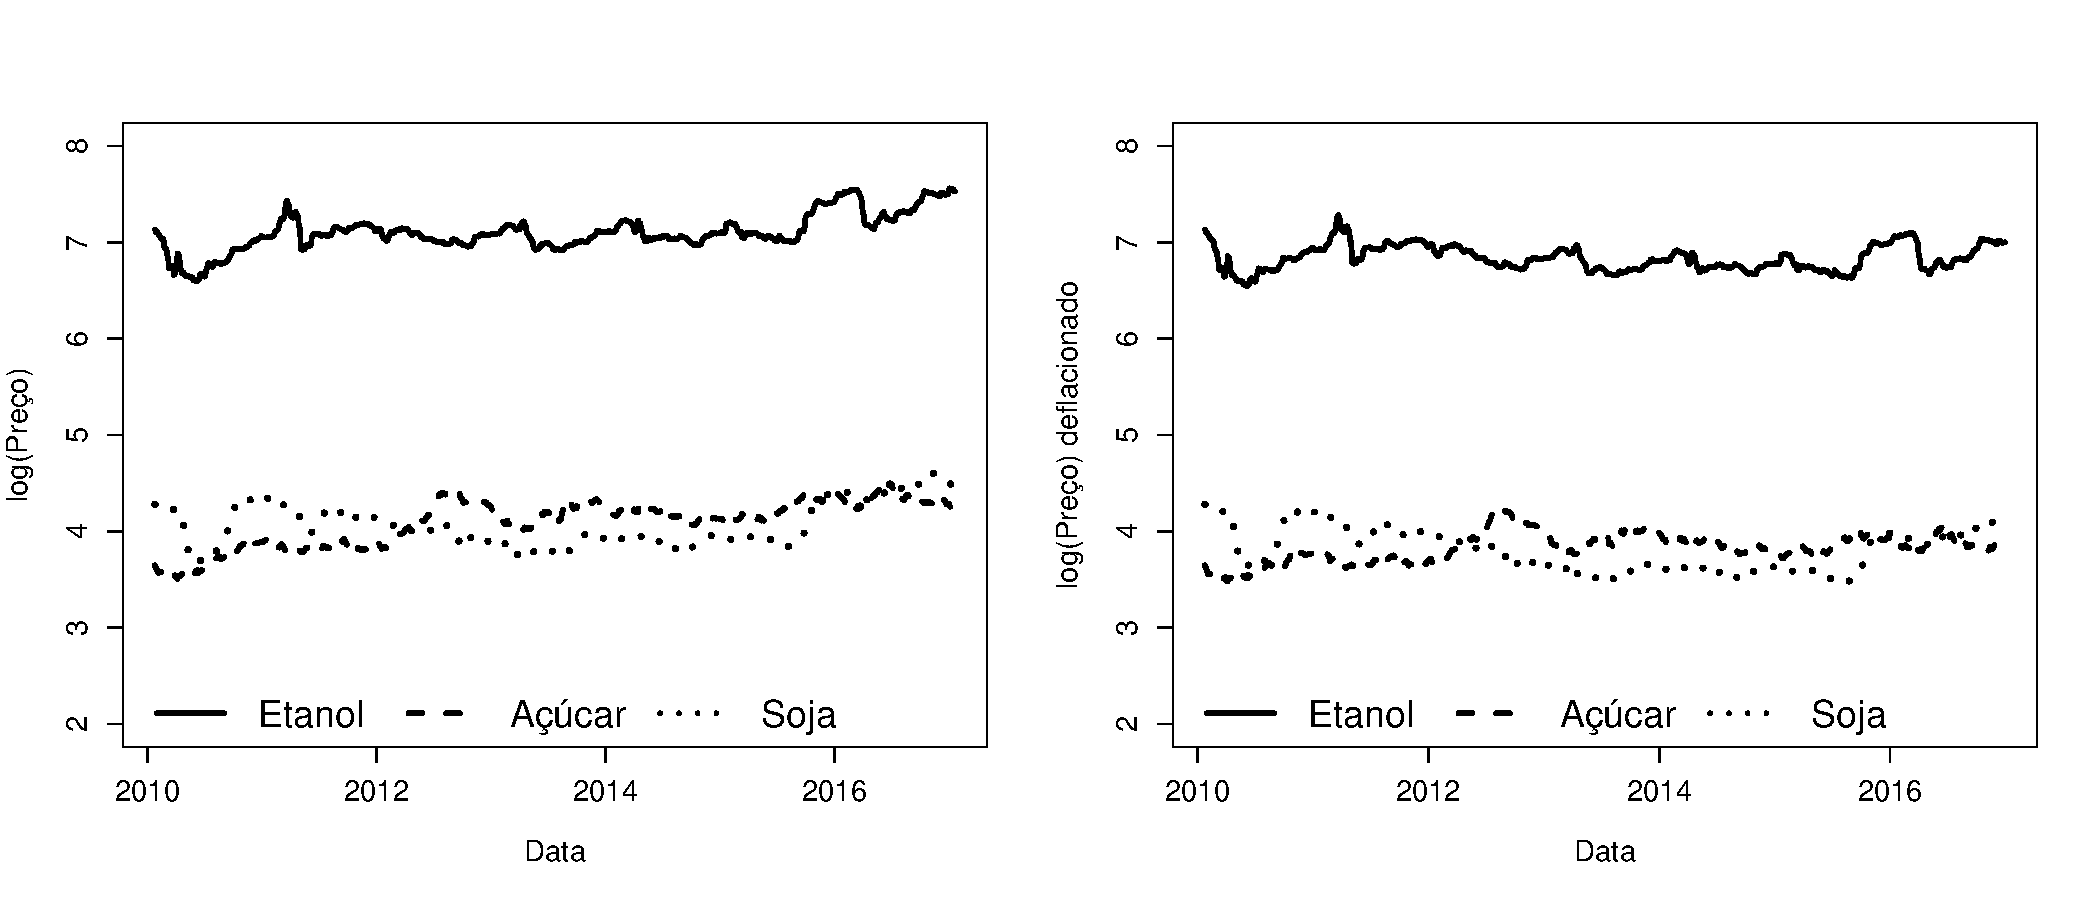
\includegraphics{grafico1-1.pdf}
\caption{Logarítimo dos preços diários e preço diário deflacionado pelo
Ìndice de Preço do Produtor (IPP) para o etanol, açúcar e soja}
\end{figure}

\begin{figure}[htbp]
\centering
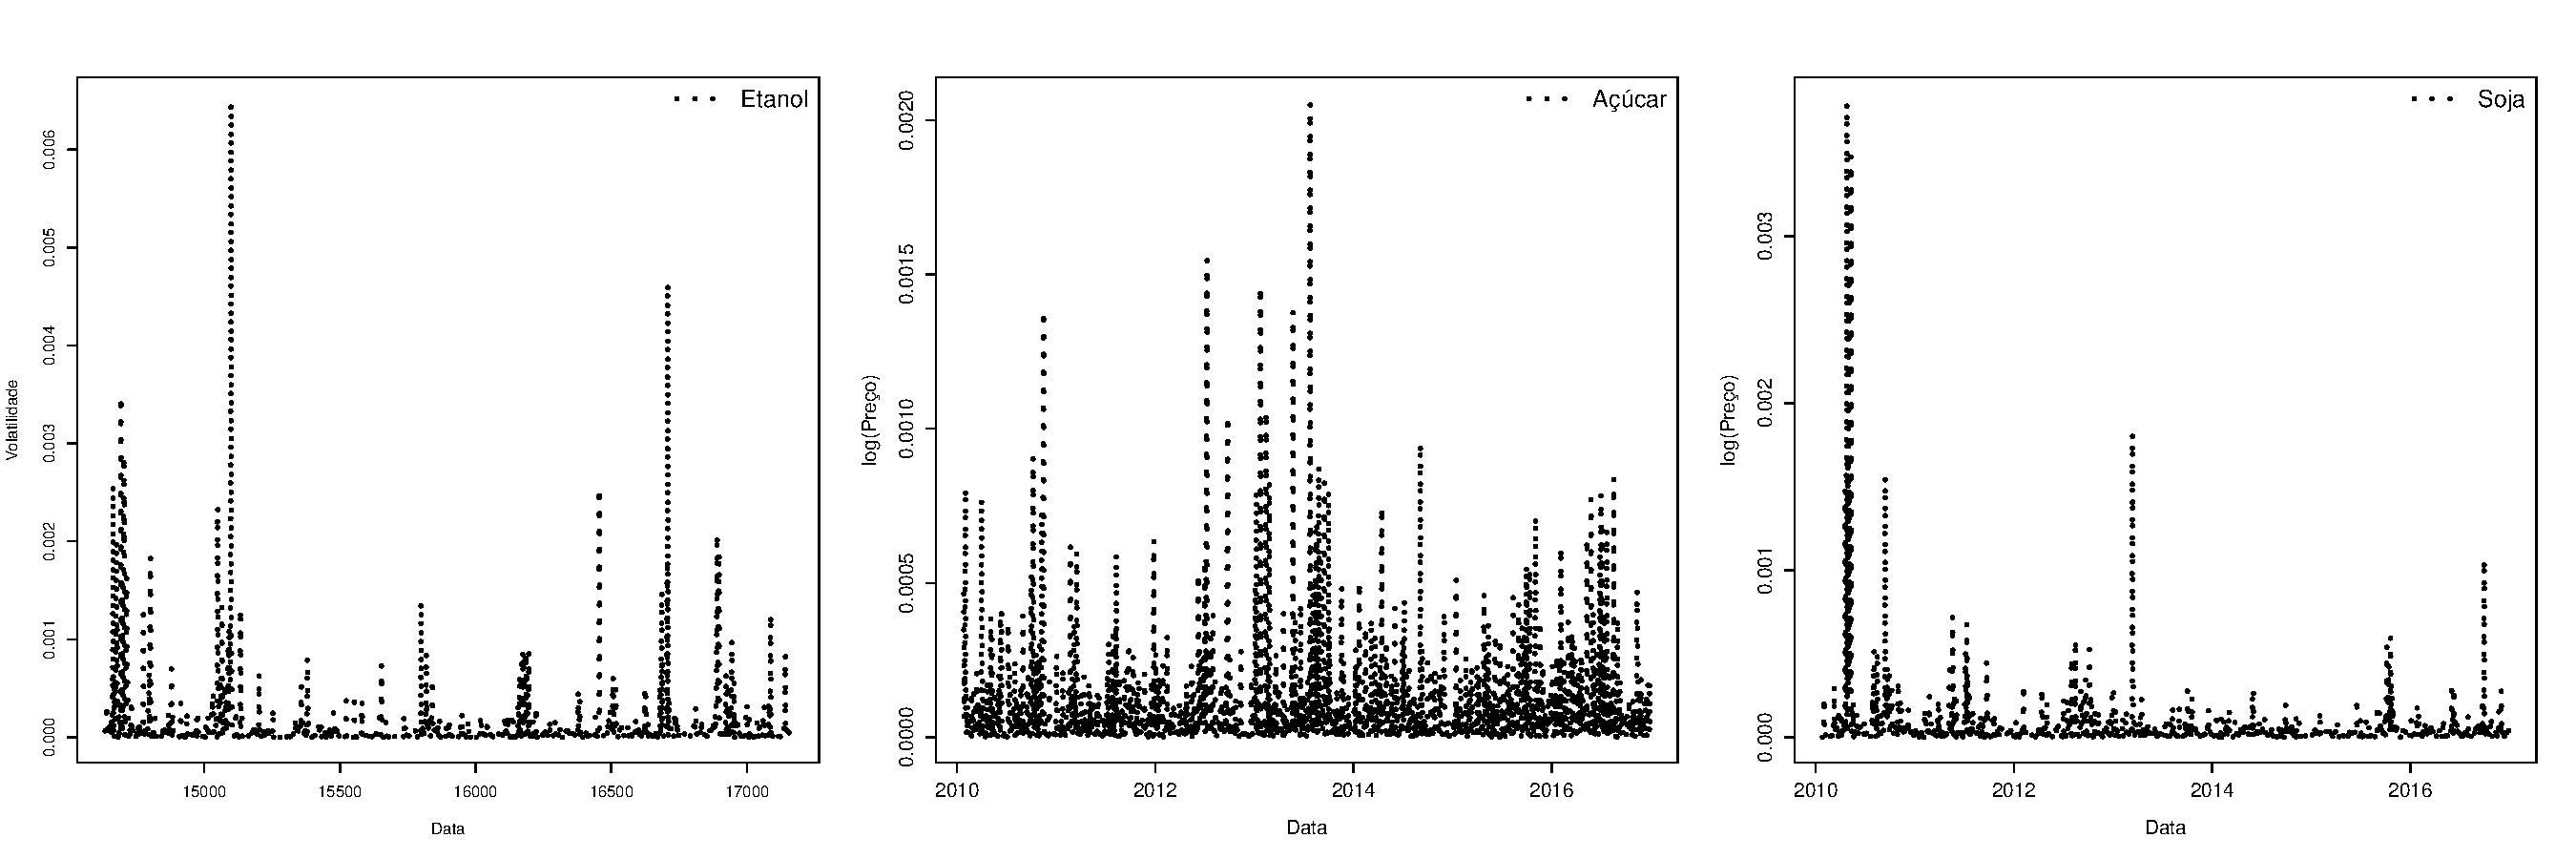
\includegraphics{grafico2-1.pdf}
\caption{Volatilidade medida pela diferença do logarítimo do preço ao
quadrado para a etanol, açúcar e soja}
\end{figure}

\pagebreak

\begin{longtable}[]{@{}lrrr@{}}
\caption{Distribuição das variáveis.}\tabularnewline
\toprule
& Etanol & Açúcar & Soja\tabularnewline
\midrule
\endfirsthead
\toprule
& Etanol & Açúcar & Soja\tabularnewline
\midrule
\endhead
Média & 938,48 & 46,35 & 45,82\tabularnewline
Desvio Padrão & 126,37 & 6,82 & 10,64\tabularnewline
& & &\tabularnewline
Correlação & 1,00 & -0,22 & 0,60\tabularnewline
& & 1,00 & -0,41\tabularnewline
& & & 1,00\tabularnewline
Assimetria & -0,29 & -0,16 & -0,06\tabularnewline
Curtose & 12,33 & 4,29 & 12,85\tabularnewline
\(Q\)(20) & \textless{}0,01 & \textless{}0,01 &
\textless{}0,01\tabularnewline
\(Q^2\)(20) & \textless{}0.01 & \textless{}0,01 &
\textless{}0,01\tabularnewline
Arch & \textless{}0,01 & \textless{}0,01 &
\textless{}0,01\tabularnewline
Shapiro-Wilk & \textless{}0,01 & \textless{}0,01 &
\textless{}0,01\tabularnewline
\bottomrule
\end{longtable}

Na Tabela 2 são apresentados a média, desvio padrão e correlações do
nível de preços do etanol, açúcar e soja. O preço do açúcar é
positivamente correlacionado com o preço do etanol, o que era de se
esperar pois os dois produtos são substitutos na perspectiva do
produtor. Por exemplo, caso o preço do etanol esteja elevado e apresente
maior lucratividade em relação ao açúcar, o produtor tende a aumentar a
oferta de etanol e reduzir a oferta de açúcar, o que por sua vez,
aumenta o preço do açúcar. A correlação entre soja e etanol é positiva.
Esta tendência explica os co-movimentos dos preços das
\emph{commodities} no mercado financeiro internacional. Quanto à
correlação negativa entre o soja e o açúcar, a análise é mais indireta
em que tal correlação pode ocorrer devido a características especulativas
inerentes do mercado financeiro.

As outras estatísticas da Tabela 2 se referem à volatilidade,
\(v_{i,t}\). As três séries apresentam assimetria à esquerda em sua
distribuição. As volatilidades de soja e etanol apresentam elevado grau
de leptocurtose (12,33 e 12,85) enquanto o nível de leptocurtose do
açúcar (4,29) é bem inferior às outras duas \emph{commodities}. Para os
testes foram reportados o valor-p. \(Q\)(20) e \(Q^2\)(20) são os testes
de Ljung-Box para \(v_{i,t}\) e \(v_{i,t}^2\) respectivamente com 20
defasagens em ambos os testes, para mais detalhes sobre o teste consulte
\citeonline{mcleod_diagnostic_1983}. Os teste \(Q\) possui hipótese nula de ausência de
autocorrelação:

\begin{equation}
 H_0: \rho_1=\rho_2=\ldots=\rho_m=0
 \end{equation}

contra a hipótese alternativa de que pelo menos um coeficiente de
autocorrelação é diferente de zero:

\begin{equation}
H_a:\exists \;\rho_i\neq 0, \quad i =1,\ldots,m
\end{equation}

Conforme \citeonline{tsay_introduction_2012}, a regra de decisão é rejeitar a hipótese nula caso
o valor-p seja inferior ao nível de significância desejado. Os testes
tanto para a \(v_{it}\) quanto para \(v_{it}^2\) possuem valor-p
inferiores a 1\% o que nos leva a rejeitar a hipótese nula de ausência
de autocorrelação para as três séries e, com isso, as volatilidades não
são independentemente distribuídas. Arch é o teste de efeitos ARCH de
Engle (1982) que é um teste de multiplicador de Lagrange para
heterocedasticidade condicional. Este teste é equivalente à estatística
\(F\) para testarmos se \(\alpha_i=0\), \(i=1,\ldots,m\), na regressão
linear

\begin{equation}
a_t^2=\alpha_0+\alpha_1a_{t-1}^2+\ldots+\alpha_ma_{t-m}^2+\varepsilon_t,\quad t=m+1,\ldots,T.
\end{equation}

Em que \(a_t=v_t-\mu_t\), ou seja, o resíduo em relação à média
condicional, \(\varepsilon_t\) é o termo de erro, \(m\) é o número de
defasagens incluídas no teste e \(T\) o tamanho da amostra. A série ao
quadrado \(a_t^2\) é usada para checar a heterocedasticidade
condicional, cujo teste possui a hipótese nula

\begin{equation}
H_0:\alpha_1=\ldots=\alpha_m=0,
\end{equation}

contra a hipótese alternativa

\begin{equation}
H_a:\exists \; \alpha_i\neq 0, \quad i=1,\ldots,m.
\end{equation}

Maiores detalhes sobre o cálculo destas estatísticas também podem ser
encontrados em \citeonline{tsay_introduction_2012}. A regra de decisão é rejeitar a hipótese nula
se o valor-p for menor que o nível de significância desejado.Portanto, no
teste de efeito ARCH rejeitou-se a hipótese nula de ausência de
heterocedasticidade condicional para as três séries a um nível de
significância de 1\%. Com isso inferimos que existe heterocedasticidade
condicional nas séries estudadas.

Para testar a normalidade dos dados realizou-se o teste Shapiro-Wilk,
inicialmente desenvolvido por \citeonline{shapiro_analysis_1965}. Este teste infere
se a amostra estudada veio de uma distribuição normal. Como os valores-p
reportados na Tabela 2 são menores que o nível de significância de 1\%,
rejeita-se a hipótese nula de que os dados foram amostrados de uma
distribuição normal. Até então todos as estatísticas estão em
conformidade com a literatura de volatilidade no mercado financeiro, em
que os dados apresentam leptocurtose, assimetria à esquerda,
heterocedasticidade condicional e não normalidade em sua distribuição.
Alguns trabalhos recentes que identificaram estas características são,
\citeonline{lopez_cabrera_volatility_2016}, \citeonline{freitas_volatilidade_2015} e \citeonline{araujo_estimacao_2015}, para uma excelente revisão sobre o assunto, veja \citeonline{serra_biofuel-related_2013}.

\subsection{Testes de estacionariedade, raiz unitária e
cointegração.}\label{testes-de-estacionariedade-raiz-unitaria-e-cointegracao.}

Em seguida foram feitos os testes Dickey-Fuller aumentado (ADF, sigla em
inglês), KPSS e Phillips-Perron para identificar se as séries de preços
possuem raiz unitária, no caso dos testes ADF e Phillips-Perron ou se as
séries de preços são estacionárias, por meio do teste KPSS. A Tabela 3
mostra as estatísticas do teste KPSS e o valor tabela por nível de
significância. Podemos ver nesta tabela que todas as estatísticas,
independente da especificação do modelo, são maiores que os valores
tabelasdos, portanto não rejeitamos a hipótese nula de estacionariedade.
As tabelas 4 e 6 mostram os testes ADF e Phillips-Perron
respectivamente. A diferença destes dois testes em relação ao teste
KPSS, é que eles possuem hipótese nula de existência de raiz unitária.
Conforme as duas tabelas 4 e 6, para qualquer especificação do modelo não
rejeitamos a hipótese nula de existência de raiz unitária nas séries
estudadas. Uma vez que evidenciamos a existência de raiz unitária nas
séries de preços, foram realizados os mesmos testes para as séries em
primeira diferença, onde constatou-se que elas são integradas em
primeira ordem. A partir disso podemos prosseguir para a identificação
de cointegração e estimação do modelo de vetor de correção de erros
(VECM, sigla em inglês).

\begin{longtable}[t]{lrrrrrrr}
\caption{\label{tab:ADF e KPSS nivel}Teste KPSS preço em nível}\\
\toprule
  & etanol & acucar & soja & 1 Pct & 2.5 Pct & 5 Pct & 10 Pct\\
\midrule
Time Trend: & 1.57 & 3.80 & 5.17 & 0.22 & 0.18 & 0.15 & 0.12\\
No Trend: & 1.88 & 10.65 & 9.45 & 0.74 & 0.57 & 0.46 & 0.35\\
\bottomrule
\end{longtable}

\begin{longtable}[t]{lrrrrrrr}
\caption{\label{tab:ADF e KPSS nivel}Teste ADF preço em nível}\\
\toprule
  & etanol & acucar & soja & 1 Pct & 2.5 Pct & 5 Pct & 10 Pct\\
\midrule
Time Trend: & -3.83 & -1.67 & -2.44 & -3.96 & -3.66 & -3.41 & -3.12\\
Constant: & -3.87 & -1.90 & -2.67 & -3.43 & -3.12 & -2.86 & -2.57\\
Neither: & -0.16 & 0.27 & -0.39 & -2.58 & -2.23 & -1.95 & -1.62\\
\bottomrule
\end{longtable}

\begin{longtable}[t]{lrrr}
\caption{\label{tab:ADF e KPSS nivel}Defasagens do teste ADF}\\
\toprule
  & Trend Model & Drift Model & None\\
\midrule
etanol & 2 & 2 & 2\\
acucar & 1 & 1 & 1\\
soja & 6 & 6 & 5\\
\bottomrule
\end{longtable}

\begin{longtable}[]{@{}lrrr@{}}
\caption{Teste Phillips-Perron}\tabularnewline
\toprule
& Z(\(\alpha\)) & Defasagem & valor-p\tabularnewline
\midrule
\endfirsthead
\toprule
& Z(\(\alpha\)) & Defasagem & valor-p\tabularnewline
\midrule
\endhead
Etanol & -18,99 & 8 & 0,09\tabularnewline
Açúcar & -6,74 & 8 & 0,07\tabularnewline
Soja & -3,90 & 8 & 0,90\tabularnewline
\bottomrule
\end{longtable}

Como critério para seleção da ordem de defasagem do modelo VAR usamos os
critério AIC, BIC e HQ. Estes testes reportaram como número de
defasagens ótimas, 7, 4 e 6, respectivamente e por uma questão de
parcimônia usamos o número de defasagens sugerido pelo critério BIC (4
defasagens). Como o número ótimo de defasagens do modelo VAR é 4, para o
teste de cointegração devemos usar 3 defasagens. O teste realizado foi o
teste do traço de Johansen que possui hipótese nula de ausência de
cointegração contra uma hipótese alternativa de cointegração entre as
variáveis. O teste do traço verifica se o posto (\emph{rank}) da matriz
de cointegração \(\Pi = \alpha \beta'\) é igual a zero. a hipótese
alternativa é a de que \(0<rank(\Pi)<n\) e \(n\) é o número máximo
possível de vetores de cointegração. Se a hipótese nula de que o posto
da matriz \(\Pi\) seja zero for rejeitada, realiza-se o teste novamente
com a hipótese nula de que o posto seja 1 e assim sucessivamente até não
se rejeitar a hipótese nula. O posto da matriz \(\Pi\) será definido
logo quando não se rejeitar a hipótese nula do teste. O número de
vetores de cointegração é igual ao posto da matriz \(\Pi\).

\begin{longtable}[]{@{}llrr@{}}
\caption{\label{johansen}Teste do traço de Johansen}\tabularnewline
\toprule
\(H_0\) & \(H_a\) & Estatística do teste & Valor crítico a
5\%\tabularnewline
\midrule
\endfirsthead
\toprule
\(H_0\) & \(H_a\) & Estatística do teste & Valor crítico a
5\%\tabularnewline
\midrule
\endhead
\(r=0\) & \(r>0\) & 42,16 & 31,52\tabularnewline
\(r\leq 1\) & \(r>1\) & 13,22 & 17,95\tabularnewline
\(r\leq 2\) & \(r>2\) & 4,12 & 8,18\tabularnewline
\bottomrule
\end{longtable}

Como se verifica na Tabela \ref{johansen}, inicialmente rejeitou-se a hipótese nula
de que o posto da matriz \(\Pi\) seja zero, em seguida não se rejeitou a
hipótese nula de que o posto seja igual a um. Logo, exite uma única
relação de cointegração dada por:

\begin{equation}\label{coint}
p_t^e-0,03\,p_t^a-0,316\,p_t^s=0
\end{equation}

em que \(P_t^e\), \(p_t^a\) e \(p_t^s\) são os preços do etanol, açúcar
e soja, respectivamente. Agora, dado o vetor de cointegração, podemos
estimar o modelo VECM para obtermos a volatilidade livre do co-movimento
entre as médias dos preços.

\subsection{Estimação do modelo de vetor de correção de
erros.}\label{estimacao-do-modelo-de-vetor-de-correcao-de-erros.}

Foi estimado um modelo de vetor de correção de erros a partir do vetor
de cointegração encontrado anteriormente. Tanto a relação de longo prazo,
quanto a dinâmica de curto prazo são capturadas por este modelo. Depois
de realizado um refinamento ao remover os coeficientes não significantes
a \(5\%\) o modelo parcimonioso ficou (erro padrão entre parênteses):

\begin{align}\label{vecm}
\Delta p_t^e &=-\underset{(0,002)}{0,01}\hat{\beta}^Tp_{t-1}+\underset{(0,024)}{0,373}\Delta p_{t-1}^e+\underset{(0,024)}{0,258}\Delta p_{t-2}^e+\underset{(0,015)}{0,061}\Delta p^s_{t-2}+\underset{(0,024)}{0,036}\Delta p^e_{t-3}+u_t,\nonumber\\
\Delta p_t^a &=-\underset{(0,002)}{0,005}\hat{\beta}^Tp_{t-1}-\underset{(0,021)}{0,057}\Delta p^e_{t-1}+\underset{(0,023)}{0,2}\Delta p^a_{t-1}-\underset{(0,017)}{0,026}\Delta p_{t-2}^s-\underset{(0,022)}{0,043}\Delta p_{t-3}^e+u_t,\\
\Delta p_t^s &=\underset{(0,023)}{0,22}\Delta p_{t-1}^s+\underset{(0,024)}{0,174}\Delta p_{t-2}^s+\underset{(0,023)}{0,23}\Delta p_{t-3}^s+u_t.\nonumber
\end{align}

em que \(\hat{\beta}^Tp_{t-1}\) é a relação de cointegração estimada na
equação \eqref{coint}. Dado que os preços são diários o conjunto de
equações em \eqref{vecm} representam as mudanças percentuais de um dia
para o outro. Com relação ao etanol, a relação de longo prazo entre as
variáveis impacta negativamente o retorno do ativo (\(\Delta p_t\)). O
retorno do etanol sofre impacto de seus componentes autorregressivos e
do retorno do soja na defasagem de segunda ordem, porém é um efeito fraco
se comparado com os componentes autorregressivos.

O retorno do açúcar também sofre impacto negativo dos co-movimento entre
as médias dos preços, assim como o retorno do etanol. Já seus
componentes autorregressivos impactam seu retorno de forma positiva, já
que o efeito autorregressivo de primeira ordem sobrepõe o efeito de
terceira ordem. O etanol impacta o retorno do açúcar de forma negativa,
fato que corrobora a relação direta de oferta entre os dois produtos.
Para o açúcar, desta-se ainda um efeito significativo do soja no termo
de segunda defasagem, porém, como para o etanol, o efeito é muito fraco
e dissipado pelos componentes autorregressivos. Por fim o retorno do
soja também possui forte impacto positivo de seus componentes
autorregressivos e não apresenta nenhuma influência significativa dos
demais retornos.

Na figura 3 estão plotados os resíduos do modelo VECM estimado com
refinamento. Visualmente fica perceptível a heterocedasticidade
condicional dos termos de erro, porém alguns teste estatísticos para
detectar a heterocedasticidade condicional ainda são necessários. Os
testes escolhidos foram os testes de Portmanteau e os teste baseados no
posto. 

\begin{figure}[htbp]
	\centering
	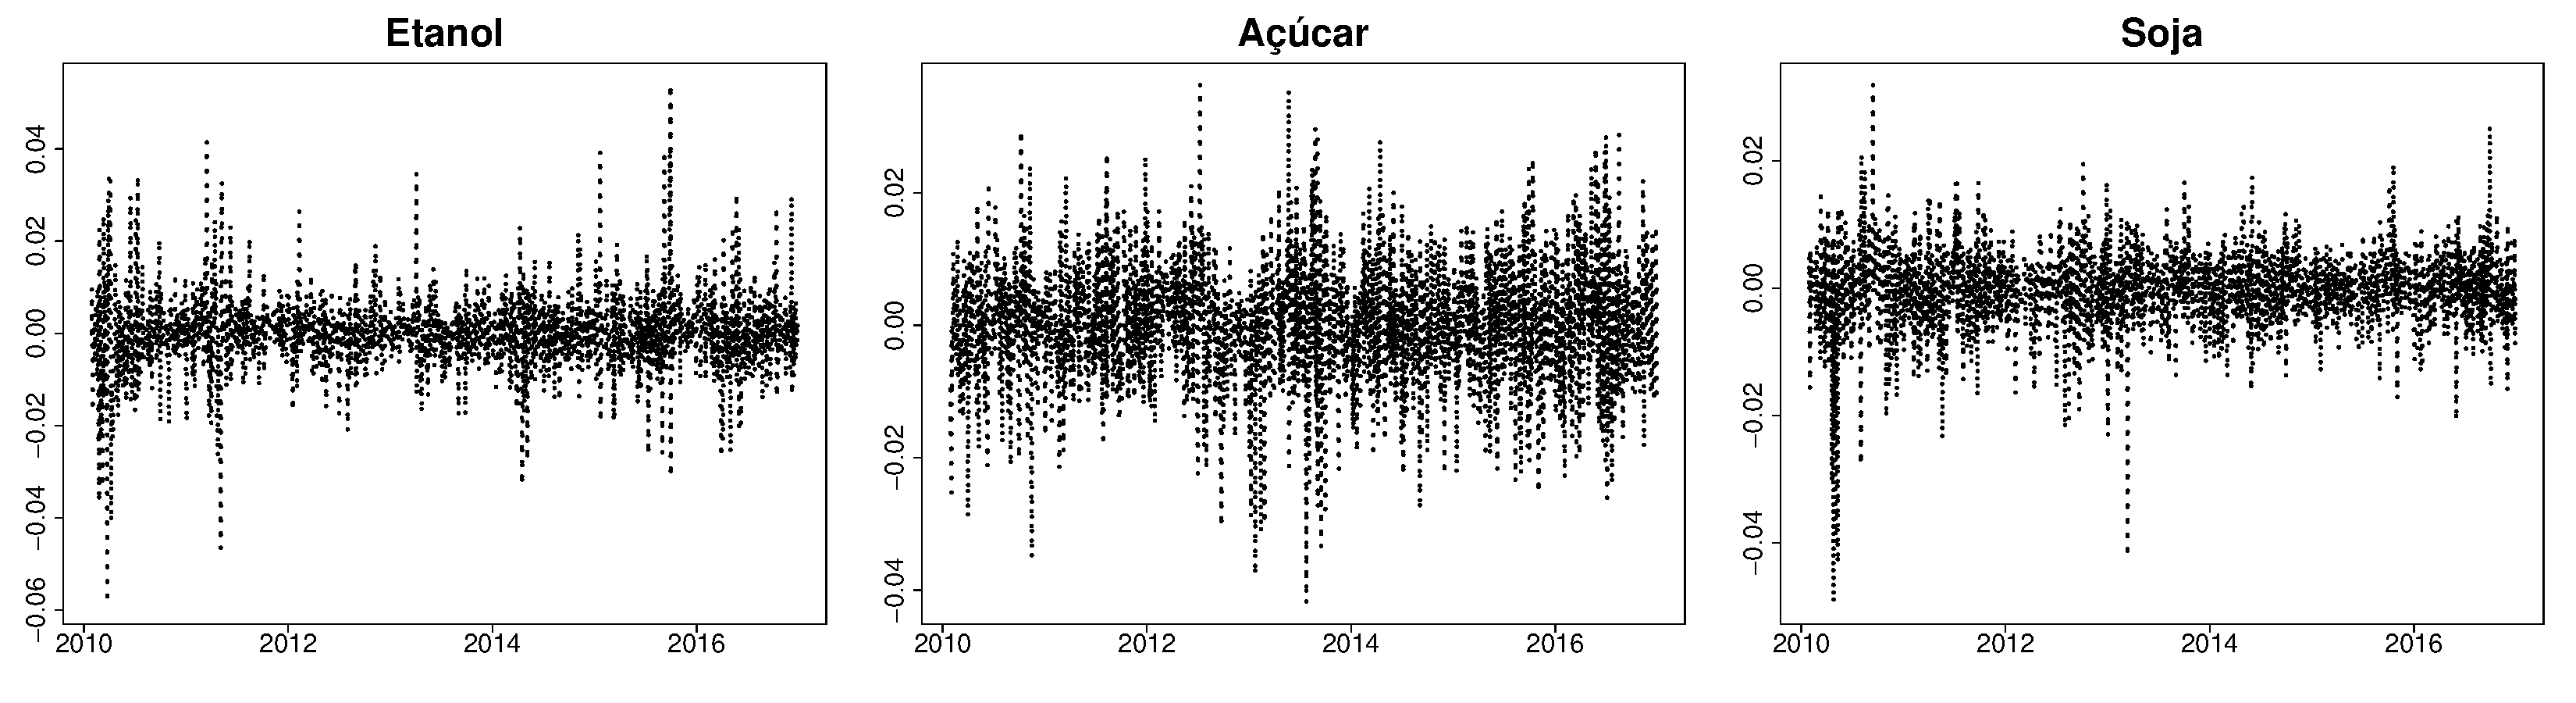
\includegraphics{VECM resid-1.pdf}
	\caption{Resíduos das estimação do modelo de vetor de correção de erros
		(VECM)}
\end{figure}

Como consta na Tabela \ref{marcht} os três primeiros testes se referem ao
teste de Portmanteau (\(Q^*_k(m)\) ) e suas extensões , a versão
ajustada para a média (\(Q^*(m)\) ) e a versão robusta com truncamento
de cauda superior de 5\% (\(Q^r_k(m)\)), e também o teste de posto
(\(Q_R(m)\)). Para mais detalhes sobre estes testes Tsay (2013) fornece
um excelente ponto de partida.



\begin{longtable}[]{@{}lllll@{}}
\caption{\label{marcht}Testes de heterocedasticidade condicional.}\tabularnewline
\toprule
& \(Q^*_k(m)\) & \(Q^*(m)\) & \(Q^r_k(m)\) & \(Q_R(m)\)\tabularnewline
\midrule
\endfirsthead
\toprule
& \(Q^*_k(m)\) & \(Q^*(m)\) & \(Q^r_k(m)\) & \(Q_R(m)\)\tabularnewline
\midrule
\endhead
Teste & 646,09 & 213,39 & 503,87 & 184,77\tabularnewline
valor-p & \textless{}0,01 & \textless{}0,01 & \textless{}0,01 &
\textless{}0,01\tabularnewline
\bottomrule
\end{longtable}

Todos os teste falharam em rejeitar a hipótese nula de ausência de
heterocedasticidade condicional a um nível de significância inferior a
1\%, como era o esperado já que observamos na Figura 3 que os dados
sugeriam a ocorrência de heterocedasticidade condicional e os dados por
se tratarem de séries financeiras possuem este comportamento. Uma vez
que foi identificada a heterocedasticidade condicional para a série de
dados podemos modelar a heterocedasticidade condicional.




\subsection{Estimação do modelo BEKK.}\label{estimacao-do-modelo-bekk.}

Na seção anterior realizou-se a estimação do modelo de vetor de correção
de erros para a obtenção do resíduo livre do co-movimento entre as
médias. Porém, ao usarmos 4 defasagens para o modelo VAR, e
consequentemente 3 defasagens para o modelo VEC, os resíduos do modelo
VEC ainda apresentaram correlação. Já que o método de estimação BEKK
proposto por \citeonline{engle_multivariate_1995} supõe que os dados sejam não
correlacionados e isso não ocorreu após a estimação do modelo VEC (os
resíduos permaneceram correlacionados) foi realizado o mesmo
procedimento anterior, mas escolhendo diferentes defasagens para o
modelo VAR. Constatamos que usando o número máximo de desafagens (7),
indicado pelo critério AIC, os resíduos do modelo VEC estimado
posteriormente não apresentam correlação serial até a vigésima
defasagem. Portanto o modelo BEKK será estimado usando os resíduos do
modelo VEC com 6 defasagens.

Com este novo número de defasagens escolhido, assim como no caso
anterior, identificamos um único vetor de cointegração (1, -0,125,
-0,358). Para sintetizar as correlações dos resíduos do modelo VEC(7),
plotamos os valores-p do teste de Ljung-Box realizado para estes
resíduos.

\begin{figure}[htbp]
\centering
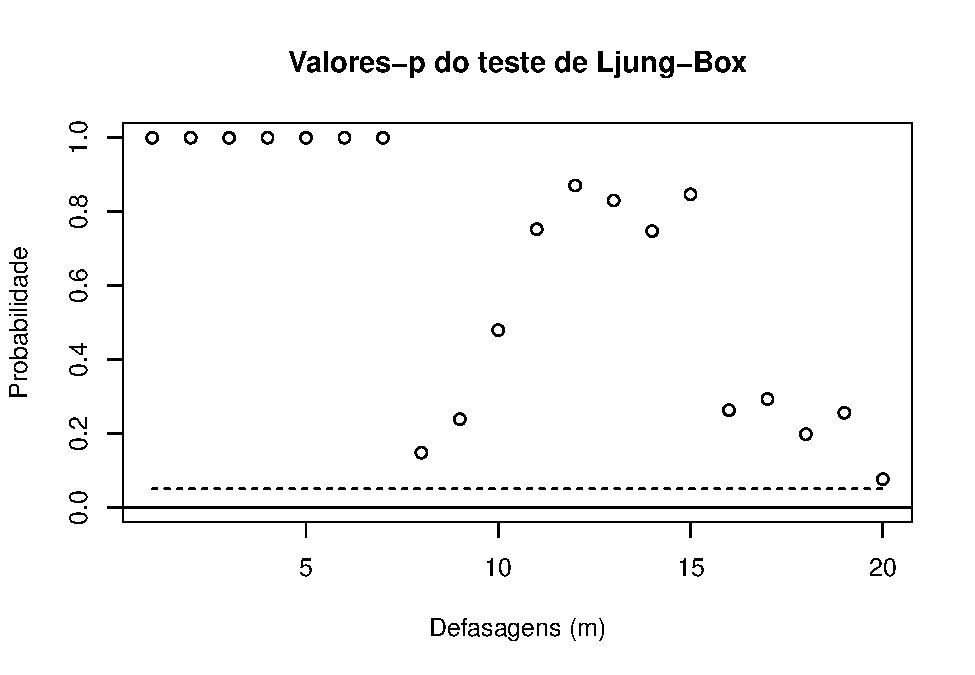
\includegraphics{mq2 test-1.pdf}
\caption{Plotagem dos valores-p das defasagens do teste multivariado de
correlação Ljung-Box.}
\end{figure}

Como podemos observar, todas os valores-p estão são maiores que 5\%
(linha tracejada). Portanto para estas defasagens não se rejeita a
hipótese nula de ausência de autocorrelação e correlação entre as
variáveis. Uma vez identificado que os resíduos não são correlacionados,
como impõe o modelo BEKK, podemos seguir adiante nas estimações.

Estimação do modelo BEKK.

\begin{verbatim}
## Initial estimates:  -3.370388e-06 9.138433e-05 -2.972673e-05 0.008118471 0.0004654883 0.0005525955 0.008979964 0.0007634438 0.006105187 0.1 0.02 0.02 0.02 0.1 0.02 0.02 0.02 0.1 0.8 0.02 0.02 0.02 0.8 0.02 0.02 0.02 0.8 
## Lower limits:  -3.370388e-05 -0.0009138433 -0.0002972673 0.001623694 9.309765e-05 0.0001105191 0.001795993 0.0001526888 0.001221037 1e-06 -0.5 -0.5 -0.5 1e-06 -0.5 -0.5 -0.5 1e-06 1e-06 -0.5 -0.5 -0.5 1e-06 -0.5 -0.5 -0.5 1e-06 
## Upper limits:  3.370388e-05 0.0009138433 0.0002972673 0.008930318 0.0005120371 0.000607855 0.00987796 0.0008397882 0.006715706 0.999999 0.5 0.5 0.5 0.999999 0.5 0.5 0.5 0.999999 0.999999 0.5 0.5 0.5 0.999999 0.5 0.5 0.5 0.999999 
## 
## Coefficient(s):
##                Estimate   Std. Error  t value   Pr(>|t|)    
## mu1.etanol -2.84925e-06  2.47352e-04 -0.01152  0.9908093    
## mu2.acucar  9.14653e-05  3.29909e-04  0.27724  0.7815925    
## mu3.soja   -3.01570e-05  2.05733e-04 -0.14658  0.8834611    
## A011        7.18811e-03           NA       NA         NA    
## A021        4.24346e-04  3.56933e-04  1.18887  0.2344910    
## A031        4.97986e-04  1.92549e-04  2.58629  0.0097017 ** 
## A022        8.14837e-03           NA       NA         NA    
## A032        7.05890e-04           NA       NA         NA    
## A033        4.89427e-03           NA       NA         NA    
## A11         9.99998e-02  4.68451e-02  2.13469  0.0327862 *  
## A21         1.99998e-02  3.27585e-02  0.61052  0.5415152    
## A31         1.99996e-02  2.29792e-02  0.87034  0.3841162    
## A12         1.99997e-02  2.67969e-02  0.74634  0.4554604    
## A22         9.99993e-02  3.03239e-02  3.29770  0.0009748 ***
## A32         1.99997e-02  1.91742e-02  1.04305  0.2969232    
## A13         1.99998e-02  3.69084e-02  0.54188  0.5879025    
## A23         1.99999e-02  4.11480e-02  0.48605  0.6269333    
## A33         9.99995e-02  3.83827e-02  2.60533  0.0091786 ** 
## B11         7.99983e-01  8.83433e-03 90.55387 < 2.22e-16 ***
## B21         1.99973e-02  1.39432e-02  1.43420  0.1515161    
## B31         1.99956e-02  5.13848e-03  3.89134 9.9692e-05 ***
## B12         1.99964e-02  1.19954e-02  1.66700  0.0955135 .  
## B22         7.99983e-01           NA       NA         NA    
## B32         1.99949e-02  3.52939e-03  5.66526 1.4680e-08 ***
## B13         1.99974e-02  1.26003e-02  1.58705  0.1125005    
## B23         1.99977e-02  1.28828e-02  1.55228  0.1205947    
## B33         7.99982e-01           NA       NA         NA    
## ---
## Signif. codes:  0 '***' 0.001 '**' 0.01 '*' 0.05 '.' 0.1 ' ' 1
\end{verbatim}

Todos os coeficientes foram positivos, o que era esperado pois o modelo
BEKK implica que a matriz de variância e covariância seja positiva
definida. Poucos coeficientes estimados se mostraram significantes, o
que significa dizer que as volatilidades passadas não têm grande impacto
sobre sua própria volatilidade corrente e sobre as volatilidades dos
preços das outras \emph{commodities}. Os efeitos que se mostraram
significativos com nível de significância de 5\% foram: Com respeito ao
impacto médio da volatilidade (matriz de covariância incondicional)
apenas o soja é impactado pelo etanol, os demais efeitos não são
significativos. Em relação aos efeitos ARCH, as três \emph{commodities}
apresentaram sofrer influência de suas próprias inovações e nenhum
efeito cruzado se mostrou significativo. Agora com respeito ao
componente autorregressivo da matriz da covariâncias (efeito GARCH),
somente o etanol se mostrou significativo com respeito à efeitos
próprios. Os efeitos cruzados GARCH ocorreram para o soja sendo
impactado tanto pelo etanol quanto pelo açúcar. Ao que sugere o modelo
BEKK estimado, somente o soja sofre impactos significativos das outras
\emph{commodities}, enquanto o açúcar e o etanol sofrem influência
apenas de suas próprias inovações e volatilidades. Outra conclusão que
se pode tirar do modelo, é que o etanol possui um efeito mais forte
sobre o soja do que o açúcar, pois o etanol afeta o soja por meio da
matriz de covariância condicional e incondicional, enquanto o açúcar
impacta o soja apenas pela matriz de covariâncias condicional.



\section{Conclusão e Comentários Finais}

Neste artigo avaliamos os transbordamentos de volatilidade entre o mercado do etanol e de commodities agrícolas no Brasil utilizando o Modelo Multivariado GARCH Baba–Engle–Kraft–Kroner (BEKK). São usados dados diários de janeiro de 2010 a dezembro de 2016 para commodities soja, etanol e açúcar. Inicialmente foi estimado um modelo de vetor de correção de erros para filtrar as séries de sua relação de longo prazo e depois modelar suas respectivas volatilidades sem a interferência do co-movimento entre as médias dos preços.

Os resultados sugerem que os preços do etanol, soja e açúcar estão relacionados por dinâmica de equilíbrio de longo prazo. Além disso, a soja é impactada pelo  preço do etanol, enquanto o contrário não é válido. Este resultado pode ser explicado pelo disputa de terras entre as culturas de cana-de-açúcar e de soja. Para a volatilidade obtemos que  somente o soja sofre impactos significativos das outras commodities, enquanto o açúcar e o etanol sofrem influência apenas de suas próprias inovações e volatilidades. Também verificamos que  o etanol possui um efeito mais forte sobre o soja do que o açúcar, pois o etanol afeta o soja por meio da matriz de covariância condicional e incondicional (efeitos de longo prazo e curto prazo), enquanto o açúcar impacta o soja apenas pela matriz de covariâncias condicional (efeito de curto prazo).

Nossos resultados têm implicações políticas importantes. Diferentemente de \citeonline{serra_volatility_2011} e \citeonline{lopez_cabrera_volatility_2016} e como \citeonline{gardebroek_energy_2013} encontramos evidências significativas de transbordamento de volatilidades do mercado do etanol para os mercados de alimentos (soja). Isso é consistente ao fato que as culturas de cana de açúcar e soja concorrem com mesmo espaço territorial no Brasil. Conclui-se que a preocupação do etanol como causa da instabilidade dos preços dos alimentos pode ser justificada pelos resultados encontrados. 

Para pesquisas futuras pretendemos usar o modelo \citeonline{herwartz_generalized_2011}  para medir as inter-relações dos preços entre as commodities. O procedimento  acomoda a heterocedasticidade na estimação da relação de cointegração, o que pode levar  a  um ganho de eficiência nas estimações. 

Como comentários finais, apesar de ter apresentado o artigo, não conseguimos realizar as estimações pelo modelo proposto por  \citeonline{herwartz_generalized_2011}, então utilizamos o modelo VECM tradicional que não controla para a heterocedasticidade das séries. Outro modelo  a ser testado é o modelo de Dinâmico de Correlação Cruzada (DCC), que seria o recíproco do modelo BEKK. O modelo BEKK sofre com o problema de dimensionalidade, sendo que estima muitos parâmetros, e um modelo com mais de três variáveis se torna complexo \cite{tsay_multivariate_2013}. Entretanto, o modelo DCC supõe que  variáveis diferentes causem o mesmo efeito nas volatilidades, o que reduz consideravelmente o número de parâmetros a ser estimados, mas empiricamente este modelo tende a não apresentar resultados significativos \cite{tsay_multivariate_2013}.
\vspace{\onelineskip}
\bibliography{bib_artigo_macroeconometria}
%\include{anexoI}
%\include{anexoII}
\end{document}
